% Author: Izaak Neutelings (November 2020)
\documentclass[border=3pt,tikz]{standalone}
\usepackage{physics}
\usepackage{tikz}
\usepackage[outline]{contour} % glow around text
\usetikzlibrary{patterns,decorations.pathmorphing}
\usetikzlibrary{decorations.markings}
\usetikzlibrary{angles,quotes} % for pic (angle labels)
\usetikzlibrary{arrows.meta}
\usetikzlibrary{bending} % for arrow head angle
\usetikzlibrary{calc}
\tikzset{>=latex}
\contourlength{1.1pt}

\colorlet{mydarkblue}{blue!40!black}
\colorlet{myblue}{blue!70!black}
\colorlet{myred}{red!65!black}
\colorlet{vcol}{green!45!black}
\colorlet{watercol}{blue!80!cyan!8!white}
\colorlet{darkwatercol}{blue!80!cyan!80!black!30!white}
\colorlet{metalcol}{blue!25!black!30!white}
\tikzstyle{piston}=[blue!50!black,top color=blue!30,bottom color=blue!50,middle color=blue!20,shading angle=0]
\tikzstyle{water}=[draw=mydarkblue,rounded corners=0.1,top color=watercol!80,bottom color=watercol!90!black,middle color=watercol!40,shading angle=20]
\tikzstyle{horizontal water}=[water,top color=watercol!90!black!90,bottom color=watercol!90!black!90,middle color=watercol!80,shading angle=0]
\tikzstyle{metal}=[draw=metalcol!10!black,rounded corners=0.1,top color=metalcol,bottom color=metalcol!80!black,shading angle=10]
\tikzstyle{vvec}=[->,very thick,vcol,line cap=round]
\tikzstyle{force}=[->,myred,very thick,line cap=round]
\tikzstyle{width}=[{Latex[length=4,width=3]}-{Latex[length=4,width=3]}]
\tikzstyle{mydashed}=[dash pattern=on 1.5pt off 1.5pt]

\begin{document}


% SURFACE TENSION in container
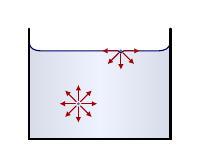
\begin{tikzpicture}
  \def\W{1.8}     % tank width
  \def\H{1.4}     % height tank
  \def\h{0.80*\H} % height water
  \def\F{0.2}     % vector magnitude
  \def\r{0.02}    % radius dot
  \def\x{0.15*\W} % x position surface dot
  \coordinate (A) at (\x,\h);
  \coordinate (B) at (-0.15*\W,0.4*\h);
  
  % WATER
  \draw[horizontal water,shading angle=90]
    (-\W/2,\h) |-++ (\W-0.007,-\h) --++ (0,\h+0.1) to[out=-90,in=0] (\W/2-0.15,\h) --
    (\x+2*\r,\h) to[out=180,in=0] (\x,\h-1.2*\r) to[out=180,in=0] (\x-2*\r,\h) --
    (-\W/2+0.15,\h) to[out=180,in=-90] (-\W/2+0.007,\h+0.1) -- cycle;
  \draw[thick,line cap=round]
    (-\W/2,\H) |-++ (\W,-\H) --++ (0,\H);
  
  % FORCES
  \fill[blue!30!black!60] (A) circle(0.02);
  \fill[blue!30!black!60] (B) circle(0.02);
  \foreach \ang in {45,90,...,360}{
    \draw[force,thin,-{Latex[length=2,width=2]}] (B)++(\ang:0.2*\F) --++ (\ang:\F);
  }
  \foreach \ang in {0,-45,...,-180}{
    \draw[force,thin,-{Latex[length=2,width=2]}] (A)++(\ang:0.2*\F) --++ (\ang:\F);
  }
  
\end{tikzpicture}


% MENISCUS CONCAVE
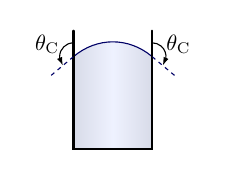
\begin{tikzpicture}
  \def\W{1.0}     % tank width
  \def\H{1.5}     % height tank
  \def\h{0.78*\H} % height water
  \def\l{0.25*\H} % length line
  \def\x{0.15*\W} % x position surface dot
  \def\ang{140}   % angle e
  \draw[horizontal water,shading angle=90]
    (-\W/2,\h) |-++ (\W,-\h) --++
    (0,\h) to[out=\ang,in=180-\ang] (-\W/2,\h) -- cycle;
  \draw[thick,line cap=round]
    (-\W/2,\H) coordinate (TL) |-++ (\W,-\H) --++ (0,\H) coordinate (TR);
  \draw[mydarkblue,mydashed] (\W/2,\h) coordinate (WR) --++ (\ang-180:\l) coordinate (R);
  \draw[mydarkblue,mydashed] (-\W/2,\h) coordinate (WL) --++ (-\ang:\l) coordinate (L);
  \draw pic[{Latex[length=3,width=2,flex'=1]}-,"$\theta_\mathrm{C}$"scale=0.8,draw=black,
            angle radius=5,angle eccentricity=2.1] {angle = R--WR--TR};
  \draw pic[-{Latex[length=3,width=2,flex'=1]},"$\theta_\mathrm{C}$"scale=0.8,draw=black,
            angle radius=5,angle eccentricity=2.1] {angle = TL--WL--L};
\end{tikzpicture}


% MENISCUS CONVEX
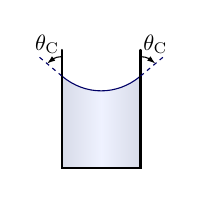
\begin{tikzpicture}
  \def\W{1.0}     % tank width
  \def\H{1.5}     % height tank
  \def\h{0.78*\H} % height water
  \def\l{0.25*\H} % length line
  \def\x{0.15*\W} % x position surface dot
  \def\ang{-140}  % angle e
  \draw[horizontal water,shading angle=90]
    (-\W/2,\h) |-++ (\W,-\h) --++
    (0,\h) to[out=\ang,in=180-\ang] (-\W/2,\h) -- cycle;
  \draw[thick,line cap=round]
    (-\W/2,\H) coordinate (TL) |-++ (\W,-\H) --++ (0,\H) coordinate (TR);
  \draw[mydarkblue,mydashed] (\W/2,\h) coordinate (WR) --++ (\ang-180:\l) coordinate (R);
  \draw[mydarkblue,mydashed] (-\W/2,\h) coordinate (WL) --++ (-\ang:\l) coordinate (L);
  \draw pic[{Latex[length=3,width=2,flex'=1]}-,"$\theta_\mathrm{C}$"scale=0.8,draw=black,
            angle radius=7,angle eccentricity=1.8] {angle = R--WR--TR};
  \draw pic[-{Latex[length=3,width=2,flex'=1]},"$\theta_\mathrm{C}$"scale=0.8,draw=black,
            angle radius=7,angle eccentricity=1.8] {angle = TL--WL--L};
\end{tikzpicture}


% SURFACE TENSION
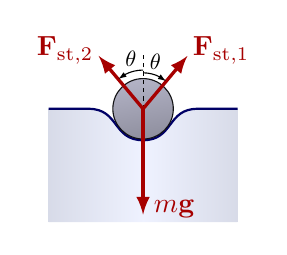
\begin{tikzpicture}
  \def\W{2.4}      % tank width
  \def\H{0.60*\W}  % height water
  \def\h{0.00*\H}  % height needle
  \def\R{0.16*\W}  % radius dot
  \def\Ry{1.8*\R}  % meniscus horizontal radius
  \def\loose{1.25} % looseness
  \def\F{3.50*\R}  % force magnitude
  \def\ang{40}     % tension angle
  \coordinate (O) at (0,\h);
  
  % WATER
  \draw[horizontal water,shading angle=90,draw=none]
    (-\W/2,0) |-++ (\W,-\H) --++ (0,\H) --
    (\Ry,0) to[out=180,in=0,looseness=\loose] (0,\h-\R-0.015)
    to[out=180,in=0,looseness=\loose] (-\Ry,0) -- (-\W/2,0) -- cycle;
  \draw[mydarkblue,thick]
    (\W/2,0) -- (\Ry,0) to[out=180,in=0,looseness=\loose] (0,\h-\R-0.015)
    to[out=180,in=0,looseness=\loose] (-\Ry,0) -- (-\W/2,0);
  
  % NEEDLE
  \draw[metal] (O) circle(\R);
  \draw[mydashed,thin] (O) -- (0,1.8*\R) coordinate (T);
  \draw[force] (O) --++ (0,-\F) node[above=2,right=0] {$m\vb{g}$};
  \draw[force] (O) --++ (90-\ang:{\F/cos(\ang)/2}) coordinate (R) node[above=2,right=-2] {$\vb{F}_\mathrm{st,1}$};
  \draw[force] (O) --++ (90+\ang:{\F/cos(\ang)/2}) coordinate (L) node[above=2,left=-2] {$\vb{F}_\mathrm{st,2}$};
  \draw pic[-{Latex[length=3,width=2,flex'=1]},"$\theta$"{scale=0.8,right=0.5,above=-1},draw=black,
            angle radius=14,angle eccentricity=1] {angle = T--O--L};
  \draw pic[{Latex[length=3,width=2,flex'=1]}-,"$\theta$"{scale=0.8,above=-1},draw=black,
            angle radius=13,angle eccentricity=1] {angle = R--O--T};
  
\end{tikzpicture}


% SURFACE TENSION - shallow
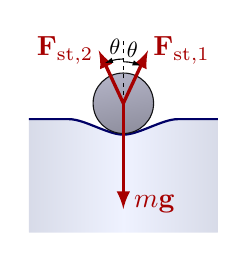
\begin{tikzpicture}
  \def\W{2.4}      % tank width
  \def\H{0.60*\W}  % height water
  \def\h{0.14*\H}  % height needle
  \def\R{0.16*\W}  % radius dot
  \def\Ry{1.8*\R}  % meniscus horizontal radius
  \def\loose{0.70} % looseness
  \def\F{3.50*\R}  % force magnitude
  \def\ang{25}     % tension angle
  \coordinate (O) at (0,\h);
  
  % WATER
  \draw[horizontal water,shading angle=90,draw=none]
    (-\W/2,0) |-++ (\W,-\H) --++ (0,\H) --
    (\Ry,0) to[out=180,in=0,looseness=\loose] (0,\h-\R-0.015)
    to[out=180,in=0,looseness=\loose] (-\Ry,0) -- (-\W/2,0) -- cycle;
  \draw[mydarkblue,thick]
    (\W/2,0) -- (\Ry,0) to[out=180,in=0,looseness=\loose] (0,\h-\R-0.015)
    to[out=180,in=0,looseness=\loose] (-\Ry,0) -- (-\W/2,0);
  
  % NEEDLE
  \draw[metal] (O) circle(\R);
  \draw[mydashed,thin] (O) -- (0,2.7*\R) coordinate (T);
  \draw[force] (O) --++ (0,-\F) node[above=2,right=0] {$m\vb{g}$};
  \draw[force] (O) --++ (90-\ang:{\F/cos(\ang)/2}) coordinate (R) node[right=-2] {$\vb{F}_\mathrm{st,1}$};
  \draw[force] (O) --++ (90+\ang:{\F/cos(\ang)/2}) coordinate (L) node[left=-2] {$\vb{F}_\mathrm{st,2}$};
  \draw pic[-{Latex[length=3,width=2,flex'=1]},"$\theta$"{scale=0.8,right=0.5,above=-1},draw=black,
            angle radius=16,angle eccentricity=1] {angle = T--O--L};
  \draw pic[{Latex[length=3,width=2,flex'=1]}-,"$\theta$"{scale=0.8,above=-1},draw=black,
            angle radius=15,angle eccentricity=1] {angle = R--O--T};
  
\end{tikzpicture}


\end{document}
